\chapter{Implémentation du M2}\label{chap:M2}
\section{Détails de la modélisation}
Construisons un méta-modèle basé sur l'entité \verb+composant+ :
\begin{itemize}
\item 
  Un \verb+composant+possède des \verb+propriétés+. Ces dernières peuvent être fonctionelles (\verb+PropFonc+) ou non fonctionelles (\verb+PropNonFonc+).
\item 
  Il possède deux interfaces composants :  une pour les \verb+services+ requis, une pour les \verb+Services+ fournis.
\item
  Une interface est aussi constituée de \verb+ports+ (fournis ou requis). 
\item
  Chaque port est associé à un et un seul \verb+service+, mais un \verb+service+ possède plusieurs \verb+ports+.  
\end{itemize}


\paragraph{}
Afin d'effectuer la communication entres composants, il est nécessaire d'introduire la notion de connecteur :

\begin{itemize}
\item 
  Un \verb+connecteur+ a deux \verb+InterfaceConnecteur+.
\item
  Chaque interface connecteur possède deux rôles : un rôle requis \verb+ roler+  et un rôle fournios \verb+rolef+ .
\item
  Chaque rôle d'une interface est relié par un lien \verb+attachement+  à son port correspondant (\textit{c.a.d }: un rôle requis à un port requis et un rôle fournis à un port fournis).  
\item
  Les deux interfaces d'un connecteur sont reliés par deux \verb+glu+  , chaque \verb+glu+  reliant un rôle requis au rôle fournis opposé.
\end{itemize}

\paragraph{}

La \verb+configuration+  est un composant composé de \verb+composants+ : 

\begin{itemize}
\item 
  Elle possède deux \verb+InterfaceConfig+. Ces dernières hériant d'\verb+InterfaceComposant+.
\item
  Il est possible de relier un \verb+portr+ de l'\verb+InterfaceConfig+ à un \verb+portr+ d'un composant de la configuration (et réciproquement pour le \verb+portf+) grâce à un lien \verb+binding+.
\item
  Un connecteur peut être aussi une \verb+configuration+.
\end{itemize}
%% \begin{description}
%% \item[G] \hfill \\
%%   Mélanges de classes de dépendances.
%% \item[Passage à l'échelle] \hfill \\
%%   Au bout d'un grand nombre de classe l'évolution et l'extension se voient limitées.
%% \end{description}
\section{Diagramme M2}
\pagestyle{empty}
\begin{figure}[htb]
  %\centering
  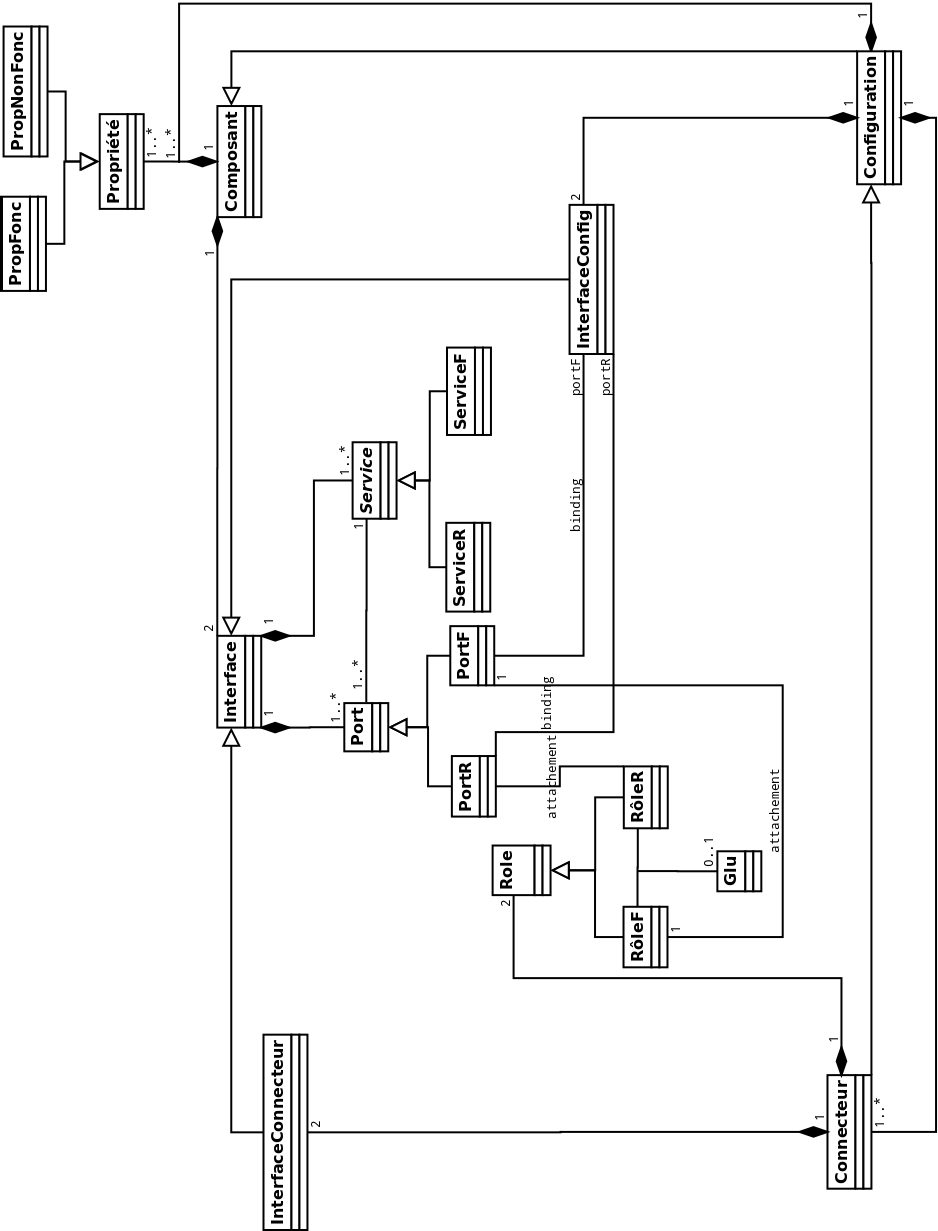
\includegraphics[scale=0.36]{img/M2}
  \caption{Méta-Model (M2)}
  \label{fig:M2}
\end{figure}
